%------------------------------------------------------------------------------
% Beginning of journal.tex
%------------------------------------------------------------------------------
%
% AMS-LaTeX version 2 sample file for journals, based on amsart.cls.
%
%        ***     DO NOT USE THIS FILE AS A STARTER.      ***
%        ***  USE THE JOURNAL-SPECIFIC *.TEMPLATE FILE.  ***
%
% Replace amsart by the documentclass for the target journal, e.g., tran-l.
%
\documentclass{amsart}

%     If your article includes graphics, uncomment this command.
\usepackage{graphicx}
\usepackage{url}
\usepackage{algorithm}
\usepackage{algorithmic}
\usepackage{amssymb}

\usepackage[backend=bibtex,
style=numeric,
bibencoding=ascii
%style=alphabetic
%style=reading
]{biblatex}
\addbibresource{journal.bib}

\newtheorem{theorem}{Theorem}[section]
\newtheorem{lemma}[theorem]{Lemma}
\newtheorem{proposition}[theorem]{Proposition}
\newtheorem{corollary}[theorem]{Corollary}

\theoremstyle{definition}
\newtheorem{definition}[theorem]{Definition}
\newtheorem{example}[theorem]{Example}
\newtheorem{xca}[theorem]{Exercise}

\theoremstyle{remark}
\newtheorem{remark}[theorem]{Remark}

\numberwithin{equation}{section}

%    Absolute value notation
\newcommand{\abs}[1]{\lvert#1\rvert}

%    Blank box placeholder for figures (to avoid requiring any
%    particular graphics capabilities for printing this document).
\newcommand{\blankbox}[2]{%
  \parbox{\columnwidth}{\centering
%    Set fboxsep to 0 so that the actual size of the box will match the
%    given measurements more closely.
    \setlength{\fboxsep}{0pt}%
    \fbox{\raisebox{0pt}[#2]{\hspace{#1}}}%
  }%
}

\begin{document}

\title{Note on reproducing kernel Hilbert spaces}

\author{Kenta Oono}
\email{k.oono.delta@gmail.com}
%    \thanks will become a 1st page footnote.
\thanks{Preferred Networks Inc.}

\maketitle

\section{notation}

\begin{itemize}
\item $A:=B$: define $A$ by $B$.
\item $\|v\|_2$: $L^2$ norm of the vector $v\in \mathbb{R}^d$.
\item vectors are represented as column vectors.
\item $\left< x, x'\right>_\mathcal{H}$: The inner product of $x$ and $x'$ in Hilbert space $\mathcal{H}$.
\item $\|x\|_\mathcal{H}$: The norm of $x$ in Hilbert space $\mathcal{H}$.
\item We only consider Hilbert space on $\mathbb{R}$.
\item $\mathrm{Span}(x_1, \ldots, x_N)= \left\{ \sum_{n=1}^{N} \alpha_n x_n \mid \alpha_n \in \mathbb{R} \right\}$
\end{itemize}

\section{Linear regression}\label{linear_regression}

\subsection{Problem setting}

Dataset $\mathcal{D} = \{ (x_1, y_1), \ldots, (x_N, y_N) \}$,
where $N = |\mathcal{D}|$ is the number of instances and
$x_i \in \mathbb{R}^d$ and $y_i \in \mathbb{R}$.
For parameter $w\in \mathbb{R}^d$, we consider the linear model.
\begin{equation}
f_w(x) := \sum_{n=1}^{N} w_n x_n = w^{T}x
\end{equation}

\begin{remark}
Normally linear model is formulated as $f(w, b) = w^{T}x + b$.
But, we can omit the bias vector $b$ by replacing $x$with $\tilde{x} = (x, 1)$.
So, we omit the bias vector from the linear model in this note.
\end{remark}

The task is to choose the most appropriate $w$ that can model the dataset from $\mathbb{R}^d$.
We evaluate the performance of the model by calculating the deviation of the
output of the model $f(x)$ from the target value $y$.
There are several choices for evaluating the deviation.
One of such metric is the $L^2$ norm defined by
\begin{equation}
l(y, y') := \frac{1}{2}(y-y')^2
\end{equation}
for $y, y'\in \mathbb{R}$.

\begin{remark}
The coefficient $\frac{1}{2}$ is not essential.
We add it to make the calculation simple.
\end{remark}

So the performance of the model is defined as
$L'(w) := \sum_{n=1}^N l(f(x_n), y_n)$.
But we do not use this function as a measure of performance.
We step one more further.
We add the penalty so that we should not choose $w$ with too large norm.
The simplest choice is to add the $L^2$ norm of the parameter $\|w\|_2^2$.
So the resulting function is
\begin{equation}
\begin{split}
L(w) &= L'(w) + \frac{\lambda}{2} \|w\|_2^2 \\
     &= \sum_{n=1}^N l(f_w(x_n), y_n) + \frac{\lambda}{2} \|w\|_2^2
\end{split}
\end{equation}
where $\frac{\lambda}{2}$ is a constant.
In the context of machine learning, a function that evaluates the performance of
the parameter like $L$ is called the \textit{loss function}
and the function like the second term of $L$ is call the \textit{regularization term}.
As both terms in $L$ are non-negative, $w$ must be chosen so that both
$f_w(x_n, y_n)$ for each $n$ and $\|w\|_2$ are small to reduce the value of $L$.
$\lambda$ regulates the effect of the second term.
The larger $w$, we reluctant to choose $w$ with large $L^2$ norm.
When $\lambda = 0$, we do not impose the penalty on the norm at all.

\begin{remark}
Different from $w$, $\lambda$ is not a tunable parameter that minimizes $L$
but rather is treated as a constant.
Such constants are called the \textit{hyper parameters}.
Tuning of hyper parameters (i.e. choice of the appropriate hyper paramters)
is out of scope of this note.
\end{remark}

\begin{remark}
$L$ implicitly depends on the dataset $\mathcal{D}$, but as we do not change the
dataset, we omit $\mathcal{D}$ from the argument for simplicity of the notation.
\end{remark}

\begin{remark}
Sometimes, we add the normalizer $\frac{1}{N}$ to the definition of $L'$.
In that case, $L'$ is often called the \textit{mean squared error}.
The essence does not change even if we introduce this coefficient because we can absorb it to the change of $\lambda$.
\end{remark}

\begin{remark}
Some of the readers may think that the choice of the form of $L$ is artificial,
but we can justify the choice of the functional form of $L$ above
from the probabilistic point of view.
Specifically, the minimization of $L$ with respect to $w$ is equivalent to
MAP estimate when we construct an appropriate probabilistic model of $w$, $x$ and $y$.
\end{remark}

\subsection{Solution}

We reformulate $L$ as follows to calculate the derivative.
\begin{equation}
L(w) = \frac{1}{2}\|Xw - y\|_2^2 + \frac{\lambda}{2} \|w\|_2^2
\end{equation}
where
\[
X =
\begin{bmatrix}
x_1^T\\
\vdots\\
x_n^T
\end{bmatrix}
=
\begin{bmatrix}
x_1^1 & \cdots & x_1^d\\
\vdots & & \vdots \\
x_n^1 & \cdots & x_n^d
\end{bmatrix}
, y = \begin{bmatrix}
y_1\\
\vdots\\
y_d
\end{bmatrix}
\]
As $L$ is quadratic in $w$, we can easily calculate the minimizer of $L$ by differentiating $L$ with respect to $w$,
by direct calculation, $\frac{\partial L}{\partial w} = X^T(Xw-y) + \lambda w$.
Setting $\frac{\partial L}{\partial w} = 0$,
\begin{equation}
\begin{split}
\frac{\partial L}{\partial x} = 0 \Leftrightarrow (X^TX+\lambda)w = X^T y.
\end{split}
\end{equation}

Note that as $X^T X$ is a symmetric positive semi-definite matrix
and $\lambda > 0$, $X^TX+\lambda$ is invertible.
So, the minimizer is 
\begin{equation}
w^{\ast} := (X^TX+\lambda)^{-1}X^Ty
\end{equation}

\subsection{Introduction of kernel functions}

Now, let's reformulate what we have done in the previous subsection.
Recall the minimizer $w^{\ast}$ should satisfy $(X^TX+\lambda)w = X^T Y$
We introduce the new variable $K$ by
\[
K = XX^T =
\begin{bmatrix}
x_1^Tx_1 & \ldots & x_n^Tx_1 \\
\vdots & & \vdots \\
x_n^T x_1 & \ldots & x_n^T x_n
\end{bmatrix}
\]
So, $K$ is a matrix that collects pair-wise inner products of $x_n$'s.
We call $K$ the \textit{Gram matrix}.
$K$ is by definition, a symmetric positive semi-definite matrix.

Also, we define $\alpha$ by $\alpha = (K+\lambda)^{-1}y$.
Note that $K+\lambda$ is invertible by the same reason as $X^TX + \lambda$.

\begin{proposition}\label{w_min}
$w^{\ast} = X^T \alpha$
\begin{proof}
\begin{equation}
\begin{split}
(X^TX + \lambda)w^{\ast} &= X^Ty \\
                  &= X^T (K+\lambda) (K+\lambda)^{-1}y \\
                  &= X^T(XX^T+\lambda) (K+\lambda)^{-1}y \\
                  &= (X^TX + \lambda)X^T (K+\lambda)^{-1}y \\
                  &= (X^TX + \lambda)X^T \alpha
\end{split}
\end{equation}
Multiplying $(X^TX + \lambda)^{-1}$ from left yields the claim.
\end{proof}
\end{proposition}

\begin{remark}
As we will see later, this relation between $w^{\ast}$ and $\alpha$ holds true in more general situation
thanks to the theorem known as Representer theorem.
\end{remark}

For a new instance $\tilde{x}$, the model predicts the target value $\tilde{y}$ by
\begin{equation}
\tilde{y} = f_w^{\ast}(\tilde{x}) = w^{\ast T} \tilde{x}
                      = (X^T \alpha)^T \tilde{x}
                      = \alpha^T X \tilde{x}
                      = \alpha^T \tilde{k}
\end{equation}
where $k$ is a collection of inner products of $x_n$'s and $\tilde{x}$
\[
\tilde{k} = X\tilde{x} =
\begin{bmatrix}
x_1^T \tilde{x}\\
\vdots \\
x_n^T \tilde{x}
\end{bmatrix}
\].

\section{nonlinearlity}

The crux here is that we need the values $\alpha$ and $\tilde{x}$,
which does not need $x_n$'s and $\tilde{x}$ themselves but their inner products
to make a prediction of new instance $\tilde{x}$.
As we do not have to handle $x_n$ directly, $x_n$'s even need not to be a vector.
It is enough for us to define the function $k: \mathcal{X} \times \mathcal{X}\to \mathbb{R}$
that works as an inner product of $x$'s
(we will show the requirements imposed to $k$ to make it be used as the substitute of the inner product).
The function $k$ is called the \textit{kernel function}.
Here, $\mathcal{X}$ is a set that works as a domain of $x$'s.
$\mathcal{X}$ need not endowed with inner product even $\mathbb{R}^d$) domain of $x$,

We substitute the inner product with $k$.

\begin{equation}
f_w^{\ast}(\tilde{x}) = \alpha^T \tilde{k}
\end{equation}
where
\begin{equation}
K =
\begin{bmatrix}
k(x_1, x_1) & \cdots & k(x_1, x_n)\\
\vdots & & \vdots \\
k(x_n, x_1) & \cdots & k(x_n, x_n)
\end{bmatrix}, \tilde{k} =
\begin{bmatrix}
k(x_1, \tilde{x})\\
\vdots\\
k(x_n, \tilde{x})
\end{bmatrix}
\end{equation}
and $\alpha = (K + \lambda)^{-1}y$.
If there exists a Hilbert space $\mathcal{H}$ and function $\phi: \mathcal{X}\to \mathcal{H}$ such that
\begin{equation}
k(x, x') = \left< \phi(x), \phi(x') \right>_\mathcal{H},
\end{equation}
then, the discussion in the previous section works by replacing $x$ with $\phi(x)$.

\begin{example}
If $\mathcal{X}$ is endowed with the inner product, we can use it to define $k$ by $k(x, x') = x^Tx'$.
We should choose $\phi(x) = x$ in this case.
Of course, we do not have to define $k$ in this way even if $\mathcal{X}$ has an inner product.
By defining more complex $k$, we can make the model $f$ more complex.
\end{example}

\begin{example}[Polynomial kernel]
Let's think of the first example of this generalization.
We define $k(x, x') = (x^Tx' + 1)^2$ for $x, x'\in X = \mathbb{R}^D$.
\begin{equation}
k(x, x') = (x^Tx' + 1)^2 = \phi(x)^T\phi(x')
\end{equation}
where $\phi(x) = (x^1x^1, \ldots x^i x^j, \ldots, x^Dx^D, \sqrt{2}x^1, \ldots \sqrt{2}x^D, 1)^T$.
So, using $k$ as an alternative of the ordinal input is equivalent to first mapping each sample $x$ to
more high-dimensional space $\mathbb{R}^{\tilde{D}}$ where $\tilde{D} = D^2 + D + 1$ by $\phi$ and consider the linear model
in $\mathcal{R}^{\tilde{D}}$.

We can generalize this discussion to the case $k(x, x') = (x^Tx' + 1)^e$ for some non-negative integer $e$.
This kernel is known as \textit{polynomial kernel}.
\end{example}

\begin{example}[RBF kernel]
We define $k(x, x') = a\exp(-b |x-x'|^2)$ for $x, x'\in \mathbb{R}^d$ where $a, b$ are hyper parameters.
We can no longer write $k(x, x')$ as the inner product of finite-dimensional vectors.
But from the general theory explained later, we can prove that there exists $\phi$ and $\mathcal{H}$ that satisfies the relation.
By considering the Taylor expansion of $k$, $\phi(x)$ should be intuitively the infinite
collection of $1, a_ix_i, b_{ij}x_ix_j, c_{ijk}x_ix_jx_k, \ldots$ where $a_i, b_{ij}, c_{ijk}$ are some constants.
This kernel is known as the \textit{RBF kernel} (Radial Basis Function kernel).
\end{example}

\begin{example}[String kernel]
This example describes that $x$ need not to be a $\mathbb{R}$-valued vector(TBD)
\end{example}

\begin{remark}
In machine learning, we often preprocess data in which we convert each raw sample into a vector that
represents the characteristic of the sample so that we can handle the data mathematically.
Such a preprocess is called \textit{feature extraction}.
From that view point, $\phi$ is sometimes called a \textit{feature map}.
\end{remark}

\begin{example}

Experiment condition of Figure \ref{experiment}.

\begin{itemize}
\item $\mathcal{D} = \left\{(x_n, y_n)\right\}_{n=1}^{100}$
\item $x_n \sim \mathrm{Unif}(-1, 1)$, i.i.d.
\item $y_n \sim \mathcal{N}(y_n \mid f(x_n), \sigma^{2})$ where $f(x) = 2 x^3 - 3 x^2 + 2x + 2$
\item $k(x, x') = \exp(-\|x-x'\|^2)$ (RBF kernel)
\item Introduce bias term $\tilde{x} = (x, 1)$
\item Regularization parameter $\lambda = 1$
\end{itemize}

\begin{figure}[tb]\label{experiment}
%\blankbox{.6\columnwidth}{5pc}
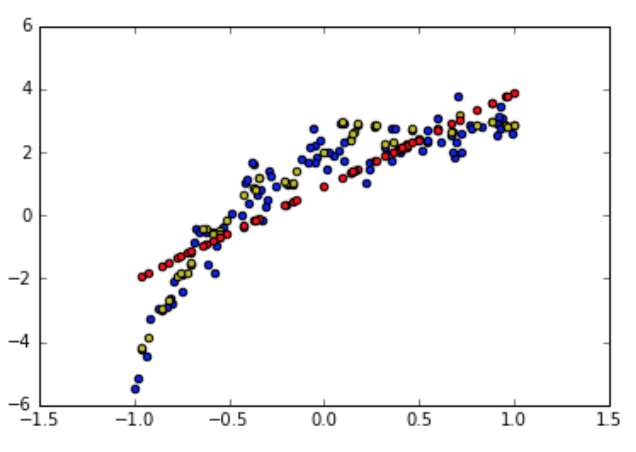
\includegraphics{kernel_regression.png}
\caption{Kernel regression. Blue: training samples. Red: Linear regression of test samples. Yellow: Regression with RBF kernel of test samples.}
\label{kernel_regression}
\end{figure}
\end{example}

\section{reproducing kernel}

In this section, we will introduce three concepts, which turned out to be equivalent.

\begin{itemize}
\item Reproducing kernels and associated Reproducing Kernel Hilbert Spaces (RKHSs).
\item Kernels
\item Symmetric positive semi-definite functions.
\end{itemize}

\subsection{Definitions}

Let $\mathcal{X}$ be a set.

\begin{definition}
A symmetric function $k: \mathcal{X} \times \mathcal{X}\to \mathbb{R}$ is \textit{positive semi-definite} if for any $N\in \mathbb{N}_{>0}$ and any $x_1, \ldots, x_N\in \mathcal{X}$, the \textit{Gram matrix}
\begin{equation}
K=
\begin{bmatrix}
k(x_1, x_1) & \cdots & k(x_1, x_n)\\
\vdots & & \vdots\\
k(x_n, x_1) & \cdots & k(x_n, x_n)
\end{bmatrix}
\end{equation}
is positive semi-definite.
\end{definition}

\begin{definition}
A symmetric function $k: \mathcal{X}\times \mathcal{X}\to \mathbb{R}$ is a \textit{kernel} if there exists a Hilbert space $\mathcal{H}$ and a function $\phi: \mathcal{X}\to \mathcal{H}$ such that
\begin{equation}
k(x, x') = \left< \phi(x), \phi(x')\right>_\mathcal{H}
\end{equation}
\end{definition}
\begin{remark}
The feature map $\phi$ in this definition is not unique in general.
\end{remark}

\begin{definition}
A symmetric function $k: \mathcal{X}\times \mathcal{X}\to \mathbb{R}$ is a \textit{reproducting kernel} if there exists a Hilbert space $\mathcal{H}$ consists of real-valued functions of $\mathcal{X}$ (i.e. $\mathcal{H}\subset \mathbb{R}^\mathcal{X}$) that satisfies the following conditions
\begin{enumerate}
\item $k(x, \cdot)\in \mathcal{H}$ for all $x$.
\item $f(x) = \left< k(x, \cdot), f\right>_\mathcal{H}$ (reproducing property).
\end{enumerate}
\end{definition}

\begin{proposition}\label{RKHS}
For a Hilbert space $\mathcal{H}$ in $\mathbb{R}^\mathcal{X}$, the followings are equivalent.
\begin{enumerate}
\item For all $x\in \mathcal{X}$, the evaluation functional $\mathrm{ev}_x: \mathcal{H}\to \mathbb{R}, \mathrm{ev}_x(f) = f(x)$ is continuous.
\item $\mathcal{H}$ has a reproducing kernel.
\end{enumerate}
\begin{proof}
(1)$\Rightarrow$(2): As $\mathrm{ev}_x$ is continuous, there uniquely exists $\phi_x\in \mathcal{H}$ such that $\mathrm{ev}_x(f) = \left<\phi_x, f\right>$ by Riesz's representation theorem.
Also, we define $k: \mathcal{X} \times \mathcal{X} \to \mathbb{R}$ by $k(x, x') = \left<\phi_x, \phi_{x'} \right>_\mathcal{H}$.
By definition, $k$ is a symmetric function on $\mathcal{X}$.
We prove that $k$ is a reproducing kernel of $\mathcal{H}$.
As $\phi_x$ itself is an element of $\mathcal{H}$, we can feed $\mathrm{ev}_{x'}$ with $\phi(x)$ for any $x'\in \mathcal{X}$ and
\begin{equation}
\phi_x(x') = \mathrm{ev}_x'(\phi_x) = \left< \phi_x, \phi_{x'} \right>_\mathcal{H} = k(x, x').
\end{equation}
Therefore, $\phi_x = k(x, \cdot)$ holds. Especially, $k(x, \cdot)\in \mathcal{H}$.
The reproducing property is proved as follows:
\begin{equation}
f(x) = \mathrm{ev}_x(f) = \left< f, \phi_x \right>_{\mathcal{H}} = \left< f, k(x, \cdot) \right>_{\mathcal{H}}.
\end{equation}
Therefore, $k$ is a reproducing kernel of $\mathcal{H}$.

(2)$\Rightarrow$(1): For all $x\in \mathcal{X}$,
\begin{equation}
|f(x)|^2 = \left<f, k(x, \cdot)\right>^2_\mathcal{H} \leq \|f\|_\mathcal{H}^2 \|k(x, \cdot)\|_\mathcal{H}^2 \to 0
\end{equation}
as $f\to 0$ in $\mathcal{H}$.
Therefore, $\mathrm{ev}_x$ is continuous.
\end{proof}
\end{proposition}

\begin{definition}
The Hilbert space $\mathcal{H}$ is called \textit{Reproducing Kernel Hilbert Space} (RKHS in short) if it satisfies one of (therefore both of) coditions in the previous proposition.
\end{definition}

\begin{remark}
We can prove that for RKHS $\mathcal{H}$, there exists an \textit{unique} reproducing kernel $k$.
\end{remark}

\subsection{Equivalence of three concepts}

\begin{proposition}
For a symmetric function $k: \mathcal{X}\times \mathcal{X}\to \mathbb{R}$, the followings are equivalent
\begin{enumerate}
\item $k$ is a reproducing kernel.
\item $k$ is a kernel.
\item $k$ is a positive semi-definite function.
\end{enumerate}
\begin{proof}
(1)$\Rightarrow$(2): We have already proved it in the proof of \ref{RKHS}.

(2)$\Rightarrow$(3): Suppose $k$ is written as $k(x, x')=\left<\phi(x), \phi(x')\right>_\mathcal{H}$ for some function
$\phi: \mathcal{X}\to \mathcal{H}$. Then, for any $N\in \mathbb{N}_{>0}$, $a=(a_1, \ldots a_N)\in \mathbb{R}^N$ and $x_1, \ldots, x_N$, we have
\begin{equation}
\begin{split}
a^TKa &= 
\begin{bmatrix}
a_1 & \cdots & a_N
\end{bmatrix}
\begin{bmatrix}
\left<\phi_1, \phi_1 \right>_\mathcal{H} & \cdots & \left<\phi_1, \phi_N \right>_\mathcal{H}\\
\vdots& &\vdots\\
\left<\phi_N, \phi_1 \right>_\mathcal{H} & \cdots & \left<\phi_N, \phi_N \right>_\mathcal{H}
\end{bmatrix}
\begin{bmatrix}
a_1 \\
\vdots \\
a_N
\end{bmatrix}\\
&=\sum_{i, j=1}^{N} a_i a_j \left< \phi_i, \phi_j \right>_\mathcal{H}  = \left< \sum_i a_i \phi_i, \sum_j a_j \phi_j \right>_\mathcal{H} \geq 0,
\end{split}
\end{equation}
were, we write $\phi_i = \phi(x_i)$ for short. The last inequality follows from the positivity of the inner product.
Therefore, $k$ is positive semi-definite.

(3)$\Rightarrow$(1): This is known as \textit{Moore-Aronszajn} theorem.
We omit the proof here, see \cite{Sejdinovic-Gretton} section 4 for the complete proof.
\end{proof}
\end{proposition}

\begin{corollary}
There is one to one correspondence between kernel functions and RKHSs in $\mathbb{R}^{\mathcal{X}}$.s
\end{corollary}

\begin{remark}
Although we do not prove Moore-Aronszajn theorem in this note, it is instructive to describe the concrete construction of the Hilbert space associated to the positive semi-definite kernel $k$.

First, we make "pre-RHKS" (we do not define this term in this note, but I think this wording is easy to convey the underlying motivation) $\mathcal{H}_0$ and extend it to the genuine RHKS by adding the limit of sequences in $\mathcal{H}$.
But we must be care the extension is a bit different from the ordinal completion to make a Hilbert space from pre-Hilbert space.

$\mathcal{H_0}$ is defined as the linear span of the function of the form $k(x, \cdot)$. 
\begin{equation}
\mathcal{H}_0 = \left\{\sum_{i=1}^{N} a_i k(x_i, \cdot) \mid N\in \mathbb{N}, a_i \in \mathbb{R}, x_i \in \mathcal{X}\right\}.
\end{equation}
We define the inner product of $f = \sum_{i=1}^{N} a_i k(x_i, \cdot)$ and $g=\sum_{j=1}^{M} b_j k(y_j, \cdot) \in \mathcal{H_0}$ by 
\begin{equation}
\left< f, g\right> := \sum_{i, j} a_i b_j k(x_i, y_j).
\end{equation}

Then, $\mathcal{H}$ consists of the function $f: \mathcal{X}\to \mathbb{R}$ which has a Cauthy sequence (with respect to the topology induced by the inner product defined above) $\{f_n\}_n$ that converge to $f$ pointwise.
We define the inner product of $\mathcal{H}$ as the limit of inner product of two Cauthy sequences in $\mathcal{H}_0$.
We can prove that
\begin{itemize}
\item $\mathcal{H}$ is a Hilbert space, that is, the inner product is well-defined and $\mathcal{H}$ is complete with respect to the norm induced by the inner product.
\item The inner product of $\mathcal{H}_0$ is indentical to that of $\mathcal{H}$ restricted to $\mathcal{H}_0$.
\item $\mathcal{H}_0$ is dense in $\mathcal{H}$.
\item $k$ is a reproducing kernel of $\mathcal{H}$.
\end{itemize}
\end{remark}

\section{Kernel method}

With the results of previous section in hand, let's generalize the linear regression problem of section \ref{linear_regression}.
Dataset $\mathcal{D} = \{ (x_1, y_1), \ldots, (x_N, y_N) \}$,
where $N$ is the number of instances and $x_i \in \mathcal{X}$ and $y_i \in \mathbb{R}$.
Let $k: \mathcal{X}\times \mathcal{X}\to \mathbb{R}$ be a positive semi-definite kernel.
From the previous discussion, there exists a Hilbert space $\mathcal{H} \subset \mathbb{R}^{\mathcal{X}}$
whose reproducing kernel is $k$ such that $k(x, \cdot)\in \mathcal{H}$ for all $x\in \mathcal{X}$ and $f(x) = \left<k(x, \cdot), f \right>_\mathcal{H}$ for all $\mathcal{H}$.
We define the feature extraction function $\phi: \mathcal{X}\to \mathcal{H}$ by $\phi(x):= k(x, \cdot)$.
Note that $k(x, x') = \left< \phi(x), \phi(x') \right>_\mathcal{H}$ for all $x, x'\in \mathcal{H}$.

\begin{remark}
As $\phi$ is not unique for fixed $k$, we choose and fix one particular $\phi$.
We will see the result does not depend on the choice of $\phi$ that satisfies $k(x, x') = \left< \phi(x), \phi(x')\right>_\mathcal{H}$.
\end{remark}

For parameter $w\in \mathcal{H}$, we consider the linear model.
\begin{equation}
f_w(x) := \left<w, \phi(x)\right>_\mathcal{H} \left(= \left<w, k(x, \cdot)\right>_\mathcal{H}\right)
\end{equation}

Let $l: \mathbb{R}\times \mathbb{R}\to \mathbb{R}$ be a function that evaluates the deviation of the prediction 
from the target value. Also we introduce the regularization of the parameter as we did in the previous problem setting.
We assume that the regularizer depends on the norm of the parameter and non-decreasing with respect to the norm.
Regularization term can be written as $R(\|w\|^2_\mathcal{H})$ for some non-decreasing function $R: \mathbb{R} \to \mathbb{R}$.
We define the loss function $L$ by the weighted sum of the error term and regularization term:
\begin{equation}
L(w) = \sum_{n=1}^{N} l(f_w(x_n), y_n) + \frac{\lambda}{2} R(\|w\|_\mathcal{H}^2)
\end{equation}
where $\lambda$ is a hyper parameter. The task is to find $w$ that minimizes $L$.

\begin{remark}
The existence nor uniqueness of the minimizer is not known in general.
So, it is enough for us to find one of the minimizers, if any.
\end{remark}

At first sight, this problem is difficult to solve because we must find the optimal parameter
from potentially infinite space $\mathcal{H}$.
But thanks to the following theorem known as \textit{Representer theorem}, we can restrict the search space 
to the finite-dimensional one.

\begin{theorem}[Representer theorem]
Let $\mathcal{H}_0 = \mathrm{Span}(\phi(x_1), \ldots, \phi(x_N))$.
Let $w \in \mathcal{H}$ and $w_0$ be the projection of $w$ to $\mathcal{H}_0$, then, $L(w_0) \leq L(w)$.
\begin{proof}
We project decompose $w$ into $w = w_0 + w_1$ where $w_0\in \mathcal{H}_0$ and $w_1 \in \mathcal{H}_0^{\perp} := \left\{ f \in \mathcal{H} \mid \left<f, g\right>_\mathcal{H}=0 \quad \forall g\in \mathcal{H}_0 \right\}$.
Then,
\begin{equation}
\begin{split}
f_w(x) &= \left< w, \phi(x) \right>_\mathcal{H}\\
       &= \left< w_0 + w_1, \phi(x) \right>_\mathcal{H}\\
       &= \left< w_0, \phi(x)\right>_\mathcal{H} + \left< w_1, \phi(x) \right>_\mathcal{H}\\
       &= \left< w_0, \phi(x)\right>_\mathcal{H} \quad \text{($\because$ $w_1 \in \mathcal{H}^{\perp}$)}\\ 
       &= f_{w_0}(x)
\end{split}
\end{equation}
The fourth line follow from the fact $w_1\in \mathcal{H}_0^{\perp}$.
Further, as $\left<w_0, w_1\right>_{\mathcal{H}} = 0$, $\|w\|_{\mathcal{H}}^{2} = \|w_0\|_{\mathcal{H}}^{2} + \|w_1\|_{\mathcal{H}}^{2}$.
In particular, $\|w\|_{\mathcal{H}}^{2} \geq \|w_0\|_{\mathcal{H}}^{2}$.
As $R$ is non-decreasing, it follows that $R(\|w\|_{\mathcal{H}}^{2}) \geq R(\|w_0\|_{\mathcal{H}}^{2})$.
Combining the two, we get $L(w)\geq L(w_0)$.
\end{proof}
\end{theorem}

Therefore, if there exists minimizers of $L$, one of them should be of the form $w=\sum_{n=1}^{N}\alpha_n \phi(x_n)$.
As $k$ is the reproducing kernel of $\mathcal{H}$, $\phi(x_n) = k(x_n, \cdot)\in \mathcal{H}$.
Therefore, $w=\sum_{n=1}^N \alpha_n \phi(x_n)\in \mathcal{H}$ for all $\alpha \in \mathbb{R}^N$.
As our goal is to find at least one minimizer, we should search for $\alpha=(\alpha_1, \ldots, \alpha_N)$, not $w$, that minimizes $L$.
From that perspective, we define $f_\alpha$ as an alternative of $f_w$ as $f_\alpha = \sum_{n} \alpha_n k(x_n, \cdot)\in \mathcal{H}$
so that $f_\alpha = \left< w, \phi(x)\right>_\mathcal{H}$ for $w = \sum_{n=1}^N \alpha_n \phi(x_n)$.
For such $w$, we can show that
\begin{equation}
\begin{split}
\|w\|_\mathcal{H}^2 &= \left<\sum_{n=1}^N \alpha_n \phi(x_n), \sum_{m=1}^N \alpha_m \phi(x_m) \right>_\mathcal{H}\\
                    &= \sum_{n, m} \alpha_n \alpha_m \left< \phi(x_n), \phi(x_m)\right>_\mathcal{H}\\
                    &= \|f_\alpha\|_\mathcal{H}^2.
\end{split}
\end{equation}

Therefore, we redefine the loss function $L$ as
\begin{equation}
L(\alpha) = \sum_{n=1}^N l(f_\alpha(x_n), y_n) + \frac{\lambda}{2} R(\|f\|_\mathcal{H}^2).
\end{equation}

\begin{remark}
$\|w\|_\mathcal{H}^2$ can be also written as $\alpha^T K \alpha$ where we again define the Gram matrix $K$ by
\begin{equation}
K=
\begin{bmatrix}
k(x_1, x_1) & \cdots & k(x_1, x_n)\\
\vdots & & \vdots\\
k(x_n, x_1) & \cdots & k(x_n, x_n)
\end{bmatrix}
.
\end{equation}
\end{remark}

\begin{remark}
The fact that one of the minimizers (if exists) can be written as the linear combination of
$\phi(x_n)$'s corresponds to the previous proposition \ref{w_min}, in which we set $\mathcal{X}=\mathcal{H}=\mathbb{R}^d, k(x, x') = x^Tx'$, and $\phi(x)=x$.
\end{remark}

\begin{remark}
The correspondence of $w\in \mathcal{H}_0$ and $\alpha\in \mathbb{R}^N$ is not 1-to-1 as $\phi$ can "collapse" the input space and send different $\alpha$'s to same $w$.
That is why we introduce new function $f_\alpha$ and redefine $L$ as a function of $\alpha$.
\end{remark}

The task we have to do is
\begin{itemize}
\item (Train) to find optimal (or at least near-optimal) $\alpha$ that minimizes $L$.
\item (Inference) to calculate $f_\alpha(x)$ with fixed $\alpha$ and $x$.
\end{itemize}
\begin{remark}
As we can see, the feature space $\phi$ does not appear in the functional form of $L$ and $f_\alpha$.
So, optimal $\alpha$ and the value of $f_\alpha$ do not depend of the choice of the feature function $\phi$.

\end{remark}

In some cases, we can explicitly calculate the minimizer of $L$ explicitly, as we see in section \ref{linear_regression}.
But in general, we cannot calculate the optimal $\alpha$ analytically (i.e. we cannot derive the explicit formula of $\alpha$).
In that case, we need to make use of some optimization method to find optimal or at least near-optimal $\alpha$.
If $l$ is convex, there exist various kind of optimization algorithms to find the minimizer of $L$.
Even if $l$ is non-convex, gradient-based algorithm sometimes achieve local optimal.
In the next note, we will derive how to approximately solve this optimization problem.


\section{Randomized algorithm for fast and memory-efficient calculation of kernels}

\subsection{motivation}

Kernel trick is a technique that elegantly introduces non-linearity to linear models without handling feature map directly.
But it requires to work on the Gram matrix of the training dataset.
For example, in the simplest case we dealt with in the previous note,
we have to calculate $\alpha = (K + \lambda)^{-1}y$, whose complexity is $O(N^3)$ computational complexity where $N$ is the number of training data.
It is prohibitive when $N$ is large.
Another example is the evaluation of $f_w(x) = \sum_{n=1}^N \alpha_n k(x_n, x)$.
It typically takes $O(ND)$ operation if $\dim\mathcal{X} = D$ (e.g. $k(x, x')=x^Tx$ or $\exp(-a\|x-x'\|^2)$).
Further, we must retain whole training dataset to make a inference of newly added test sample.

Inference is equivalent to calculate $f_w(x) = \left< w, \phi(x)\right>_\mathcal{H}$ for new sample $x$, as we do in the linear regression, which is prohibitive in general because $\phi(x)$ is typically high dimensional, or possibly
infinite dimensional.
But if we could approximate the feature map $\phi$ with the (not necessarily injective) embedding to the low dimensional space $z: \mathcal{X}\to \mathbb{R}^S$, where $\dim\mathcal{X} \gg S$,
we can use it to construct a linear classifier $f_{\tilde{w}}(x) := \tilde{w}^Tz(x)$, it drastically decrease the operation cost to typically $O(D+S)$, which is independent of $N$.

So the goal is to find the approximation of feature map so that, the following approximation holds:
\begin{equation}
k(x, x') = \left<\phi(x), \phi(x') \right>_\mathcal{H} \approx z(x)^Tz(y).
\end{equation}

In this section, we restrict ourselves to translation-invariant kernel on $\mathcal{X} = \mathbb{R}^D$,
i.e. a kernel function $k$ that satisfies $k(x, x') = k(x-a, x'-a)$ for all $x, x', a \in \mathbb{R}^D$.
By setting $\psi(x):= k(x, 0)$, $k$ is written as $k(x, x')=\psi(x-x')$.
Conversely, even function $\psi: \mathbb{R}^D\to \mathbb{R}$ defines a symmetric function $k$.

\begin{remark}
When we consider $\mathbb{R}^D$ an abelian group by ordinal addition.
$\mathbb{R}^D$ acts on $L^2(\mathbb{R}^D\times \mathbb{R}^D)$ by translation,$a\cdot k(x, x'):= k(x-a, x'-a)$.
Translation-invariant kernel is a fixed point of this action.
\end{remark}

\subsection{Random Fourier Feature}

Rahimi and Recht proposed in \cite{rahimi2007random} that fast and memory efficient
approximation of the feature function. Schematically, they made use of the following calculation.
\begin{equation}
k(x, x') = C \int \zeta_\omega(x) \zeta_\omega^{\ast}(x') p(\omega) \mathrm{d}\omega 
\end{equation}


The following theorem known as Bochner's theorem is the key for our algorithm.

\begin{theorem}[Bochner's theorem]
For continuous even function $\psi:\mathbb{R}^D \to\mathbb{R}$ such that $\psi(0)=1$, we define symmetric function $k(x, x'):=\psi(x-x')$.
$k$ is a kernel function if and only if $\psi$ is a real-valued characteristic function for some probability measure.
\begin{proof}
"If" part is easy to derive.
Let $\mu$ be a probability measure and write $\psi(x)$ as $\int \zeta_\omega(x) \mathrm{d}\mu(\omega)$
where $\zeta_\omega(x) := \exp(\sqrt{-1}\omega^Tx)$.
Let $N\in \mathbb{N}_{>0}$, $a=(a_1, \ldots, a_N)\in \mathbb{R}^N$, and
$x_1, \ldots, x_N\in \mathbb{R}^N$.
We set $K=(k(x_i, x_j))_{i, j=1}^N = (\psi(x_i-x_j))_{i, j}$.
Then,
\begin{equation}
\begin{split}
a^TKa &= \sum_{i, j=1}^{N} a_i a_j \psi(x_i-x_j)\\
      &= \sum_{i, j}a_i a_j \int \zeta_\omega(x_i-x_j)\mathrm{d}\mu(\omega)\\
      &= \sum_{i, j}a_i a_j \int \zeta_\omega(x_i) \zeta_\omega^{\ast}(x_j)\mathrm{d}\mu(\omega)\\
      &= \int \left| \sum_i a_i \zeta_\omega(x_i) \right|^2 \mathrm{d}\mu(\omega)\geq 0,
\end{split}
\end{equation}
\begin{equation}
\psi(0) = \int 1 \mathrm{d}\mu(\omega) = 1.
\end{equation}

\begin{equation}
\begin{split}
\psi(-x) &= \int \zeta_\omega(-x) \mathrm{d}\mu(\omega) \\
         &= \int \zeta_\omega^{\ast}(x) \mathrm{d}\mu(\omega) = \psi^{\ast}(x).
\end{split}
\end{equation}
As $\psi$ is real-valued, $\psi(-x) = \psi(x)$, i.e. $\psi$ is symmetric.

See e.g. \cite{Sun} Theorem 1.1 for the proof of "only if" part.
\end{proof}
\end{theorem}

By conbining the case $k(x, x')=\psi(x-x')\not = 1$, we can write $k$ as
\begin{equation}
\begin{split}
k(x, x') &= \psi(0) \int \zeta_\omega(x-x') \mathrm{d}\mu(\omega)\\
         &= \psi(0) \int \zeta_\omega(x) \zeta_\omega^{\ast}(x') \mathrm{d}\mu(\omega)
\end{split}
\end{equation}
Further, if there exists a distribution $p$ such that $p(w)\mathrm{d}\omega = \mathrm{d}\mu(\omega)$
(e.g. $\mu$ is absolutely continuous with respect to Lebesgue measure),
we can estimate the value of $k$ by sampling from the distribution $f$
\begin{equation}
k(x, x') \approx \frac{1}{S} \sum_{s=1}^S \zeta_{\omega_s}(x) \zeta_{\omega_s}^{\ast}(x'),
\end{equation}
where $S$ is the number of samples and $\omega_s \sim p$.
Therefore, we can employ $z(x) =
\frac{1}{\sqrt{S}} \left[ \zeta_{\omega_{1}}(x), \ldots, \zeta_{\omega_{S}}(x) \right]^T$ as the approximation of the feature function.
\cite{dai2014scalable} listed other examples of kernel functions that we can explicitly write and sample from the corresponding distributions.

\begin{remark}
As $\zeta_{\omega}(x)$ is complex-valued. We usually use $(\cos(\omega^Tx), \sin(\omega^Tx))\in \mathbb{R}^2$ instead.
We will use both of them interchangeably in this note.
\end{remark}

\begin{remark}
For later use, We rewrite $z(x)$ as $z(x) = \frac{1}{\sqrt{S}}\exp(\sqrt{-1}\Omega x)$ where $\Omega = [\omega_{1}, \ldots, \omega_{S}]$ and $\exp$ is applied in a element-wise way.
\end{remark}

The Fourier transform and its inverse is defined as
\begin{equation}
\begin{split}
\mathcal{F}f(\omega) &:= \frac{1}{(\sqrt{2\pi})^D}\int f(x) \zeta_\omega^{\ast}(x) \mathrm{d}x\\
\check{\mathcal{F}}g(x) &:= \frac{1}{(\sqrt{2\pi})^D}\int g(\omega) \zeta_\omega(x) \mathrm{d}\omega.
\end{split}
\end{equation}
where $f, g \in \mathcal{L}^{1}(\mathbb{R}^D)$.
We will write $\hat{f} := \mathcal{F}f$ and $\check{g}:=\check{\mathcal{F}}g$ for short.
If $\psi\in \mathcal{L}^{1}(\mathbb{R}^D)$ and its Fourier transform $\hat{\psi}$ is also in $\mathcal{L}^{1}(\mathbb{R}^D)$, we can use $\hat{\psi}$ to define the measure in the Bochner's theorem. As
\begin{equation}
\begin{split}
k(x, x') &= \psi(x-x')\\
&= \check{\mathcal{F}}\mathcal{F}f(x-x')\\
&= \int \mathcal{F}f(w) \zeta_{w}(x-x')\mathrm{d}w\\
&= \int \mathcal{F}f(w) \zeta_{w}(x) \zeta_{w}^{\ast}(x') \mathrm{d}w,
\end{split}
\end{equation}
we should take $d\mu(w) \propto \mathcal{F}f(w)\mathrm{d}w$.

\begin{example}
In some specific case, we can explicitly write the functional form of $\mu$ and sample from it.
Consider RBF kernel $k(x, x')=\exp(-a\|x-x'\|^2)$ for $a > 0$.
Where we can explicitly write the Fourier transform of $\psi$ as
\begin{equation}
\hat{\psi}(\omega) = \frac{1}{(\sqrt{2a})^D} \exp \left(-\frac{\omega^2}{4a}\right).
\end{equation}
By properly choosing the normalizing constant, we obtain
\begin{equation}
k(x, x') = \psi(0) \int \zeta_\omega(x)\zeta_\omega^{\ast}(x') p(\omega)\mathrm{d}\omega
\end{equation}
where $p(\omega) = \frac{1}{(\sqrt{4\pi a})^D}\exp\left(-\frac{\|\omega\|^2}{4a} \right)$.
\end{example}

\begin{algorithm}
\caption{Random Fourier Feature}
\begin{algorithmic}
\REQUIRE Kernel function $k: \mathbb{R}^D \times \mathbb{R}^D\to \mathbb{R}$
\REQUIRE Sampling number $S$
\ENSURE Approximated feature map: $z: \mathbb{R}^D\to \mathbb{R}^S$ s.t. $z(x)^Tz(x')\approx k(x-x')$
\STATE Calculate $p(\omega)$ from $k$
\STATE Sample i.i.d. $\omega_s$ from $p$ for $s=1, \ldots S$
\STATE $z(x) := \frac{1}{\sqrt{S}}[\zeta_{\omega_1}(x), \ldots, \zeta_{\omega_S}(x)]$
\end{algorithmic}
\end{algorithm}

\cite{rahimi2007random} analyzed the asymptotic behavior of this randomized feature map and proved
that the approximated kernel converges to the true kernel on compact set of $\mathbb{R}^D\times \mathbb{R}^D$.
\cite{sriperumbudur2015optimal} proved more sharp convergence rate of this approximated feature map.
See \cite{rahimi2007random} Claim 1 and \cite{sriperumbudur2015optimal} Theorem 1 for detail.


The following proposition shows that using Random Fourier Feature and constructing linear predictor
is almost equivalent to restricting search space in RKHS.
\begin{proposition}[\cite{yang2012nystrom} Proposition 1]
Let $\mathcal{H}_{\mathrm{RFF}} = \mathrm{Span}\left\{ S_s, C_s \mid s = 1, \ldots, S \right\}$ where $S_s(x) = \sin (\omega_s^Tx)$ and $C_s(x) = \cos (\omega_s^Tx)$.
The optimization problem
\begin{equation}
\min_{f \in \mathcal{H}_{\mathrm{RFF}}} \sum_{n=1}^N l(f(x_n), y_n) + \lambda \|f\|^2_\mathcal{H}
\end{equation}
is equivalent to the following optimization problem:
\begin{equation}
\min_{w \in \mathbb{R}^{2S}} \sum_{n=1}^N l(f_w(x_n), y_n) + \lambda R(w)
\end{equation}
where $f_w(x) = w^T z(x)$ and $R(w) = \sum_{s=1}^{S} w_{2s-1}^2 \sin(\omega_s^Tx) + w_{2s}^2 \cos(\omega_s^Tx)$.
\end{proposition}

\subsection{Mercer's Theorem}
There is another justification of this approximation by sampling from the distribution on frequency with Mercer's theorem\cite{mercer1909functions}.
The following statement is from \cite{fukumizu2008}.

Let $(\mathcal{X}, \mathcal{B}, \mu)$ be a measure space where $\mathcal{X}$ is a compact Hausdorff space and $\mu$ is a finite measure. Suppose that $L^2(\mathcal{X}, \mu)$ is separable (i.e. it has countable orthogonal basis).
Let $k: \mathcal{X}\times \mathcal{X}\to \mathbb{R}$ be a continuous reproducing kernel.
We define $T_k$ as
\begin{equation}
(T_kf)(x) = \int k(x, x')f(x')\mathrm{d}x'
\end{equation}
Then $T_k$ is a linear bounded operator on $\mathrm{L}^2(\mathcal{X}, \mu)$.

\begin{theorem}[Mercer's theorem]
There exists an sequence of positive eigenvalues $\left\{\lambda_i\right\}_{i=1}^\infty$ and eigenfunctions $\left\{\varphi_i\right\}_{i=1}^\infty$ of $T_k$ such that
$\lambda_1 \geq \lambda_2 \geq \cdots \geq 0$ and 
$\lim_{i\to 0} \lambda_i = 0$.
Further, $k(x, x')$ can be expanded as
\begin{equation}
k(x, x') = \sum_{i=1}^\infty \lambda_i \phi(x)\phi^\ast(x')
\end{equation}
where the convergence is absolute and uniform.
\end{theorem}
We can show that $\left\{ \lambda_i \right\}$ is in $\ell^2(\mathbb{R})$.
Suppose $T_k$ is a Trace-class operator, $\left\{\lambda_i\right\}$ is in $\ell^1(\mathbb{R})$, then $p(i) = \frac{\lambda_{i}}{\|\lambda\|_1}$ defines the probability measure on $\mathbb{N}$.
Therefore, by sampling from this distribution, we can approximate the reproducing kernel $k$ as the inner product $k(x, x') \approx z(x)^T z(x')$ where
\begin{equation}
z(x) = \frac{\|\lambda\|_1}{\sqrt{S}} \left[ \varphi_{i_1}(x), \ldots, \varphi_{i_S}(x) \right]^T
\end{equation}
where $i_s\sim p(i)$ for $s = 1,\ldots, S$.

\subsection{Fastfood}

In RFF, we first create random matrix $V$ by sampling each element from Gaussian distribution independently and make approximate feature vector by $z(x) = \frac{1}{\sqrt{S}} \exp (\sqrt{-1}Vx)$.
Fastfood \cite{le2013fastfood} is a technique of the fast calculation of Random Fourier Feature by devising the calculation of matrix $V$.
We first assume $D = S = 2^L$ for some $L\in \mathbb{N}_{>0}$.
Fastfood calculates $V$ by
\begin{equation}
V = \frac{1}{\sigma \sqrt{D}} SHG\Pi HB
\end{equation}
where
\begin{itemize}
\item $\Pi$ is a permutation matrix.
\item $H$ is a Walsh-Hadamard matrix.
\item $G$ is a diagonal matrix such that $G_{ii} \sim \mathcal{N}(0, 1)$.
\item $S$ is a diagonal matrix $S_{ii} = s_i \|G\|_{F}^{-1/2}$ where $p(s_i) \propto s_{i}^{S-1} \exp(-s_i^2/2)$
\item $B$ is a diagonal matrix such that $B_{ii}\sim \{\pm 1\}$ uniformly random.
\end{itemize}
Walsh-Hadamard matrix is defined inductively as follows:
\begin{equation}
H_1 = 
\begin{bmatrix}
1 & 1\\
1 & -1
\end{bmatrix},
H_{2d} = 
\begin{bmatrix}
H_d & H_d\\
H_d & -H_d
\end{bmatrix}.
\end{equation}
We can easily show that $BB^T = I$, $HH^T=DI$, $\Pi \Pi^T = I$.
The calculation cost of $z(x)$ is $O(D\log d)$ rather than $O(Dd)$ by making use of FFT-like calulation of Walsh-Hadamard transform (See \cite{le2013fastfood} Lemma 6 for detail).

\begin{theorem}[\cite{le2013fastfood} Lemma 7]
$\mathbb{E}[z^{\ast}(x) z(x')] = \exp(-\frac{\|x-x'\|}{2\sigma^2})$
\begin{proof}
See \cite{le2013fastfood} Lemma 7.
\end{proof}
\end{theorem}


\section{Optimization of the loss function of kernel regression}

In this section, we consider the training of kernel machines.
In order to explain fast and efficient learning of kernel machines, known as doubly stochastic functional gradient, we will explain first gradient descent (GD) and stochastic gradient descent (SGD).


\subsection{Gradient Descent}

Consider some objective function $L:\mathbb{R}^D \to \mathbb{R}$.
Gradient descent is an optimization algorithm in which we iteratively update parameter
toward the most steepest direction.
\begin{equation}
\theta \leftarrow \theta - \eta \nabla_\theta L(\theta)
\end{equation}
where $\eta > 0$ is a small constant the detemines the step size of each iteration.

\begin{algorithm}
\caption{Gradient Descent}
\begin{algorithmic}
\REQUIRE Object function $L:\mathbb{R}^D \to \mathbb{R}$
\REQUIRE Initial parameter $\theta_0 \in \mathbb{R}^D$
\REQUIRE Step size $\eta_t \in \mathbb{R}$
\REQUIRE Time length $T$
\ENSURE optimized parameter $\theta$
\STATE $\theta \leftarrow \theta_0$
\FOR {$t = 1, \ldots T$}
\STATE $\theta \leftarrow \theta - \eta_t \nabla_\theta L(\theta)$
\ENDFOR
\STATE Return $\theta$ (or $\overline{\theta} = \frac{1}{T}\sum_{t=0}^{T-1} \theta_{t}$)
\end{algorithmic}
\end{algorithm}

\begin{remark}
In some context, $\eta$ is called the \textit{learning rate}.
\end{remark}

\begin{remark}
$\eta$ need not to be constant during whole training process.
It can be changed over iterations. i.e. schematically, $\eta = \eta_t$.
Typically, we set $\eta_t$ so that $\lim_{t\to \infty}\eta_t = 0$, $\sum_{t=1}^{\infty} \eta_t = \infty$ and $\sum_{t=1}^{\infty} \eta_t^{2} < \infty$ because there are several cases where we can theoretically prove that the algorithm converges to the local (or sometimes global) minimum. See also Robbins-Monro algorithm \cite{robbins1951stochastic}, although it should be categorized as stochastic algorithm, which we will explain in the next section.
\end{remark}

The following theorem is one of the theoretical justifications of the gradient descent algorithm.

\begin{theorem}[\cite{shalev2014understanding} Corollary 14.2]
Suppose $L$ is differentiable, convex and $\|\nabla L \| \leq \rho$.
Let $\theta^{\ast}$ be the minimizer of $L$.
Suppose $\| \theta^{\ast} \| \leq B$ and $\| \theta_{0} \| \leq B$. Then, running the gradient descent algorithm with $\eta = \sqrt{\frac{2B^2}{\rho^2 T}}$ yields the output $\overline{\theta}$ with
\begin{equation}
L(\overline{\theta}) - L(\theta^{\ast}) \leq \sqrt{\frac{2}{T}}B\rho.
\end{equation}
\begin{proof}
As $L$ is convex,
\begin{equation}\label{eq1}
L(\overline{\theta}) - L(\theta^{\ast}) = L\left(\frac{1}{T} \sum_{t=0}^{T-1} \theta_t\right) - L(\theta^{\ast}) \leq \frac{1}{T} \sum_{t=0}^{T-1} \left( L(\theta_t) - L(\theta^{\ast}) \right).
\end{equation}
Again, as $L$ is convex,
\begin{equation}
\begin{split}
& L(\theta^{\ast}) \geq L(\theta_t) + (\theta^\ast - \theta_t)^T \nabla_{\theta} L(\theta_t)\\
\Leftrightarrow & L(\theta_t) - L(\theta^\ast) \leq (\theta_t - \theta^{\ast})^T \nabla_{\theta} L(\theta_t).
\end{split}
\end{equation}
The right hand side can be transformed as follows:
\begin{equation}
\begin{split}
(\theta_t - \theta^{\ast})^T \nabla_{\theta} L(\theta_t)
&= \frac{1}{2\eta} \cdot 2(\theta_t - \theta^{\ast})^T \eta\nabla_{\theta}L(\theta_t)\\
&= \frac{1}{2\eta} \left( -\|\theta_t - \eta\nabla_{\theta}L(\theta_t) - \theta^{\ast}\|^2 + \|\theta_t - \theta^{\ast}\|^2 + \eta^2 \|\nabla_{\theta}L(\theta_t)\|^2 \right)\\
&= \frac{1}{2\eta} \left( -\|\theta_{t+1} - \theta^{\ast}\|^2 + \|\theta_t - \theta^{\ast}\|^2 + \eta^2 \|\nabla_{\theta}L(\theta_t)\|^2\right).
\end{split}
\end{equation}
By concatenating these formulae, we get
\begin{equation}\label{eq3}
\begin{split}
\sum_{t=0}^{T-1} \left( L(\theta_t) - L(\theta^{\ast}) \right)
&\leq \frac{1}{2\eta}  \sum_{t=0}^{T-1} \left( -\|\theta_{t+1} - \theta^{\ast}\|^2 + \|\theta_t - \theta^{\ast}\|^2 + \eta^2 \|\nabla_{\theta}L(\theta_t)\|^2\right)\\
&= -\frac{1}{2\eta}\|\theta_{T+1} - \theta^{\ast}\|^2 + \frac{1}{2\eta}\|\theta_1 - \theta^{\ast}\|^2 + \frac{\eta}{2}\sum_{t=0}^{T-1} \|\nabla_{\theta}L(\theta_t)\|^2\\
&\leq \frac{1}{2\eta}\|\theta_1 - \theta^{\ast}\|^2 + \frac{\eta}{2}\sum_{t=0}^{T-1} \|\nabla_{\theta}L(\theta_t)\|^2.
\end{split}
\end{equation}
As $\|\theta_1 - \theta^{\ast}\|^2 \leq 2(\|\theta_1\|^2 + \|\theta^{\ast}\|^2) \leq 2 B^2$ and $\|\nabla_{\theta}L(\theta_t)\|^2 \leq \rho^2$,
\begin{equation}
\begin{split}
\text{(RHS of \ref{eq3})} \leq \frac{1}{\eta}B^2 + \frac{\eta}{2}T\rho^2 \leq \sqrt{2T} B\rho.
\end{split}
\end{equation}
The second equality holds when $\eta = \sqrt{\frac{2B^2}{\rho^2 T}}$.
With (\ref{eq1}), we get $L(\overline{\theta}) - L(\theta^{\ast}) \leq \sqrt{\frac{2}{T}} B\rho$.
\end{proof}
\begin{remark}
The gradient descent works even if $L$ is non-differentiable. In that case, the gradient should be replaced with the subgradient and the condition on the norm of the derivative should be replaced with Lipchitz continuity condition.
\end{remark}
\end{theorem}


\subsection{Stochastic Gradient Descent}

Sometimes it is computationally prohibitive to calculate the derivative $\nabla_\theta L$.
For example, suppose $L$ is of the form
\begin{equation}
L(\theta) = \sum_{n=1}^{N} L_\theta(x_n)
\end{equation}
where $x_n$ is $n$-th sample, then, the derivative with respect to $\theta$ is
\begin{equation}
\nabla_\theta L(\theta) = \sum_{n} \nabla_\theta L_\theta (x_n).
\end{equation}
The loss function we consider so far is in this case because we should take
$L_\theta$ as $l(f_\theta (x_n), y_n)$, where we slightly abuse the notation.
The computational cost is typically $O(N)$, which is prohibitive when
the size of the data set is enormous (e.g. ImageNet\cite{imagenet_cvpr09} dataset consists of more than 14 million images).

Stochastic Gradient Descent is the algorithm that alleviate this problem
by estimating the derivative by computationally cheap method.
Specifically, we use the random variable $\xi$ that is easy to calculate and use it as the substitute of the derivative.
Typically, the random variable is \textit{unbiased} estimate of the derivative in the sense that the expectation of $\xi$ equals to the derivative of the loss function:
\begin{equation}
\mathbb{E}\left[ \xi \right] = \nabla_{\theta} L(\theta).
\end{equation}

\begin{algorithm}
\caption{Stochastic Gradient Descent}
\begin{algorithmic}
\REQUIRE Objective function $L:\mathbb{R}^D \to \mathbb{R}$
\REQUIRE Initial parameter $\theta_0 \in \mathbb{R}^D$
\REQUIRE Step size $\eta_t \in \mathbb{R}$
\REQUIRE Time length $T$
\ENSURE optimized parameter $\theta$
\STATE $\theta \leftarrow \theta_0$
\FOR{$t=1, \ldots, T$}
\STATE Sample $\xi$, the estimate of $\nabla_\theta L(\theta)$.
\STATE $\theta \leftarrow \theta - \eta_t \xi$
\ENDFOR
\end{algorithmic}
\end{algorithm}

\begin{example}
Let's consider the previous example
\begin{equation}
L(\theta) = \frac{1}{N}\sum_{n=1}^N l(f_\theta(x_n), y_n),
\end{equation}
where we have introduced the normalizer $1/N$ to make the calculation simple.

The derivative is
\begin{equation}
\nabla_{\theta}L(\theta) = \frac{1}{N}\sum_{n} l'(f_\theta(x_n), y_n) \nabla_{\theta}f_\theta(x_n)
\end{equation}

Instead of calculate the derivative for all samples $(x_n, y_n)$,
we sample the subset of the dataset $\mathcal{B} = \left\{(x_{n_1}, y_{n_1}), \ldots, (x_{n_B}, y_{n_B})\right\}$ uniformly random from the dataset and estimate the derivative by
\begin{equation}
\xi = \frac{1}{B} \sum_{b=1}^{B} l'(f_\theta(x_{n_b}), y_{n_b}) \nabla_{\theta}f_\theta(x_{n_b}).
\end{equation}
It is easy to check that $\xi$ is unbiased estiamte of the derivative of $L$ with respect to the parameter $\theta$: $\mathbb{E}_{\mathcal{B}}[\xi]=\nabla_{\theta}L(\theta)$.
At the extreme, if we sample only single sample from the dataset $\mathcal{D}$, the estimate is 
\begin{equation}
\xi = l'(f_\theta(x_n), y_n) \nabla_\theta f_\theta(x_n),
\end{equation}
where $n\sim \mathrm{Unif}([N])$

In order to calculate $\xi$, it is necessary to calculate the derivative of $f_\theta$
with respect to $\theta$ for each sample $x_n$. One of such situations is that $f_\theta$ is realized as a neural network whose weights aree parameterized by $\theta$. We can calculate the derivative by the well-known \textit{back propagation} algorithm \cite{rumelhart1988learning}.
\end{example}

\begin{remark}
Sometimes, the random variable $\xi$ is an unbiased estimate of not only the \textit{training} loss but also the \textit{generalization} loss.
Suppose we assume that the trainine dataset $\mathcal{D} = \left\{x_1, \ldots, x_N\right\}$ is sampled i.i.d. from some (unknown) distribution $\mathcal{P}$:
$x_n \sim \mathcal{P}$. The training loss $L$ is defined as
\begin{equation}
L(\theta) = \sum_{n=1}^{N} L_\theta(x_n),
\end{equation}
where $L_\theta$ is the loss function for one sample, parameterized by $\theta$,
while the generalization error $\tilde{L}$ is
\begin{equation}
\tilde{L}(\theta) = \mathbb{E}_{x\sim \mathcal{P}}\left[ L_\theta(x) \right]
\end{equation}
The unbiased estimate $\xi$ of the derivative of the (training) loss in the previous example is also the unbiased estimate of the generalization loss as well.
\end{remark}

\subsection{Optimization problem in RKHS}

For the kernel $k:\mathcal{X}\times \mathcal{X}\to \mathbb{R}$, consider again the optimization problem
\begin{equation}
L(f) = \sum_{n=1}^{N} l(f(x_n), y_n) + \frac{\lambda}{2} \|f\|_{\mathcal{H}}^2
\end{equation}
where $\mathcal{H}$ is the RKHS of $k$, $l:\mathbb{R}\to \mathcal{R}$, $\lambda > 0$, and $\mathcal{D}=\left\{(x_1, y_1), \ldots, (x_N, y_N))\right\}$.
In order to apply (S)GD to this optimization problem,
we need to calculate the derivative of $L$ with respect to $f$.
As this is a functional derivative, we use the Fr\'echet derivative instead of ordinal derivative.

\begin{definition}
Let $\mathcal{H}$ be a Hilbert space.
$\nabla L(f) \in \mathcal{H}$ is the Fr\'echet derivative of functional $L:\mathcal{H}\to \mathbb{R}$ at $f$ if 
\begin{equation}
L(f + \epsilon g) = L(f) + \epsilon \left<\nabla L(f), g\right>_\mathcal{H} + O(\epsilon^2)
\end{equation}
for all $g\in \mathcal{H}$ and $\epsilon > 0$.
\begin{remark}
We can prove that the Fr\'echet derivative is unique if it exists.
\end{remark}
\begin{remark}
For Banach space $\mathcal{B}$, Fre\'chet derivative is usually defined as the bounded linear operator on $\mathcal{B}$.
When $\mathcal{B}$ is a Hilbert space, we can convert the bounded linear operator to the element of $\mathcal{B}$ by the Riesz's representational theorem.
\end{remark}
\end{definition}

As $\mathrm{ev}_x(f) = f(x) = \left<f, k(x, \cdot) \right>_\mathcal{H}$, 
$\nabla f(x) \left( = \nabla \mathrm{ev}_x(f) \right) = k(x, \cdot)$.
Also, as $\|f + \epsilon g\|^2_{\mathcal{H}} = \|f\|_\mathcal{H}^2 + 2\epsilon \left<f, g\right>_\mathcal{H} + \epsilon^2\|g\|_\mathcal{H}^2$,  we can show that $\nabla \|f\|_\mathcal{H}^2 \left( = \nabla \|\cdot\|_\mathcal{H}^2 (f)\right) = 2f$.
Therefore,
\begin{equation}
\nabla L(f) = \sum_{n=1}^N l'(f(x_n), y_n)k(x_n, \cdot) + \lambda f,
\end{equation}
where $l'$ is the (sub)gradient of $l$.

\begin{remark}
In fact, we do not have to consider the differentiation on possibly infinite dimensional space $\mathcal{H}$ if we only have to find at least one of the minimizers thanks to the Representer theorem. But we follow \cite{dai2014scalable} and introduce the funtional derivative.
\end{remark}

\subsection{Doubly Stochastic Gradient}

Doubly Stochastic Gradient \cite{dai2014scalable} is a technique to apply the gradient descent to the optimization problem on RKHS by sampling from training dataset (as we did in SGD) and from frequency (as we did in Random Fourier Feature).
As we did in RFF, we assume that the kernel $k$ is translation-invariant and decompose the kernel function $k$ as
\begin{equation}
k(x, x') = \phi(0) \mathbb{E}_{\omega \sim p} \left[ \zeta_\omega(x) \zeta_\omega^{\ast}(x')\right]
\end{equation}
from now on, we normalize $k(x, x) = \phi(0) = 1$.
We estimate the derivative $\nabla L(f)$ with 
\begin{equation}
\xi = l'(f(x), y)\zeta_\omega(x)\zeta_\omega^{\ast}.
\end{equation}
It is straight forward to see that $\mathbb{E}_{(x, y)\sim \mathcal{D}, \omega \sim p} \left[\xi\right] = \nabla L(f)$.

\begin{remark}
Be aware that in general $\xi \not \in \mathcal{H}$. But $\mathbb{E}[\xi] \in \mathcal{H}$ as it equals to $\nabla L(f)$.
\end{remark}
Therefore, the naive algorithm is like Algorithm \ref{DSG}.
\begin{algorithm}\label{DSG}
\caption{Doubly Stochastic Gradient}
\begin{algorithmic}
\REQUIRE Objective function $L$
\REQUIRE Translation invariant kernel $k$
\REQUIRE Step size $\eta_t$
\REQUIRE Time length $T$
\ENSURE Optimized predictor $f$
\FOR{$t=1, \ldots T$}
\STATE sample $(x, y)$ uniformly from $\mathcal{D}$
\STATE sample $\omega$ from $p$
\STATE $\xi = \phi(0) l'(f(x), y)\zeta_\omega(x)\zeta_\omega^{\ast} + f$
\STATE $f \leftarrow f - \eta_t \xi$
\ENDFOR
\end{algorithmic}
\end{algorithm}
But we need more consideration to implement Algorithm \ref{DSG} because it is not obvious how to paramete
rize a function $f$.
As we look at the algorithm, we notice that $f$ must be of the form $\sum_{n:finite} \alpha_n \zeta_{\omega_n}^{\ast}$ during the optimization process.
We also notice that we add the term of the form $\alpha \zeta_{\omega} $ in each iteration. So we write $f$ of this form and update $\alpha$'s in each iteration.

\begin{algorithm}\label{DSG2}
\caption{Doubly Stochastic Gradient}
\begin{algorithmic}
\REQUIRE Objective function $L$
\REQUIRE Translation invariant kernel $k$
\REQUIRE Step size $\eta_t$
\REQUIRE Time length $T$
\ENSURE Optimized predictor $f$
\FOR{$t=1, \ldots T$}
\STATE sample $(x, y)$ uniformly from $\mathcal{D}$
\STATE sample $\omega_t$ from $p$
\STATE $f_x = \sum_{t'=1}^{t-1} \alpha_{t}\zeta_{\omega_{t}}^{\ast}$
\STATE $\alpha_t \leftarrow -\phi(0) l'(f_x, y)\zeta_\omega(x)$
\STATE $\alpha_{t'} \leftarrow (1-\eta_{t})\alpha_{t'} \quad \text{for $1\leq t' \leq t$}$
\ENDFOR
\STATE Return $f = \sum_{t=1}^T \alpha_{t}\zeta_{\omega_{t}}^{\ast}$
\end{algorithmic}
\end{algorithm}
We use $\omega_{t'}$ for $t'< t$ in iteration $t$ to calculate $f_x$.
One of the straight forward way to do so is to memorize all $\omega_t$'s.
Another way is to to use \textit{pseudo random generator}, which returns same random value for the same seed.
The drawback of this algorithm is that its complexity is $O(T^2)$ as we have to calculate $f_x$ in every iteration, which takes $O(t)$ in interation $t$.

\printbibliography

\end{document}

%------------------------------------------------------------------------------
% End of journal.tex
%------------------------------------------------------------------------------
